\documentclass{article}
\usepackage{times}
\usepackage[utf8]{inputenc}
\usepackage[T1]{fontenc}
\usepackage[russian]{babel}
\usepackage[a4paper, total={6in, 8in}]{geometry}
\usepackage{dirtytalk}
\usepackage{graphicx}
\usepackage{hyperref}
\usepackage{listings}
\usepackage{color,soul}

\graphicspath{ {./img/} }

% code listings settings
\definecolor{lightgray}{rgb}{.9,.9,.9}
\definecolor{darkgray}{rgb}{.4,.4,.4}
\definecolor{purple}{rgb}{0.65, 0.12, 0.82}

\lstdefinelanguage{JavaScript}{
	keywords={break, case, catch, continue, debugger, default, delete, do, else, false, finally, for, function, if, in, instanceof, new, null, return, switch, this, throw, true, try, typeof, var, void, while, with},
	morecomment=[l]{//},
	morecomment=[s]{/*}{*/},
	morestring=[b]',
	morestring=[b]",
	ndkeywords={class, export, boolean, throw, implements, import, this},
	keywordstyle=\color{blue}\bfseries,
	ndkeywordstyle=\color{darkgray}\bfseries,
	identifierstyle=\color{black},
	commentstyle=\color{purple}\ttfamily,
	stringstyle=\color{red}\ttfamily,
	sensitive=true
}

\lstset{
	language=JavaScript,
	backgroundcolor=\color{lightgray},
	columns=fullflexible,
	basicstyle=\ttfamily,
	extendedchars=false,
	showstringspaces=false,
	showspaces=false,
	numbers=left,
	numberstyle=\footnotesize,
	numbersep=9pt,
	tabsize=2,
	breaklines=true,
	showtabs=false,
	captionpos=b
}


\begin{document}
\title{Лабораторная работа 1}

\date{\today}
\maketitle

\say{Когда кто-то говорит: «Я хочу язык программирования, который может делать все, что ему скажу», то я даю этому человеку леденец.
	— Alan J. Perlis}

\section{Введение}

Цель: изучить структуру и работу BlockChain


\section{Основные понятия}


\begin{itemize}
	\item BlockChain (блокчейн) - выстроенная по определённым правилам непрерывная последовательная цепочка блоков (связный список), содержащих информацию. Чаще всего копии цепочек блоков хранятся на множестве разных компьютеров независимо друг от друга. 
	\item 
	\item 	
\end{itemize}


\section{Основная часть}

Основная концепция блокчейна довольно проста: распределенная база данных, которая поддерживает постоянно растущий список упорядоченных записей. 

Однако, многоe остается непонятным, если говорить о блокчейне, так же остается много проблем, которые пытаются решить с его помощью. Это относится и к популярным блокчейн проектам, таким как Биткоин (Bitcoin) и Эфириума (Ethereum). Термин "блокчейн" обычно сильно привязан к концепции типа денежных переводов, смарт-контрактов или криптовалюты. Это делает понимание блокчейна сложнее, чем есть на самом деле.

Далее будет показана реализация простого блокчейна на языке  \hl{TypeScrypt}. Он был выбран так как является очень похожим на язык \hl{Solidity}, который будет необходимо изучить для последней лабораторной.

\subsection{Структура блока}


Первый логический шаг — определиться со структурой блока. Чтобы оставить все как можно проще, включим только самое необходимое: индекс, отметка, данные, хэш и хэш предыдущего блока (Рис. 1).


\begin{figure}
	\centering
	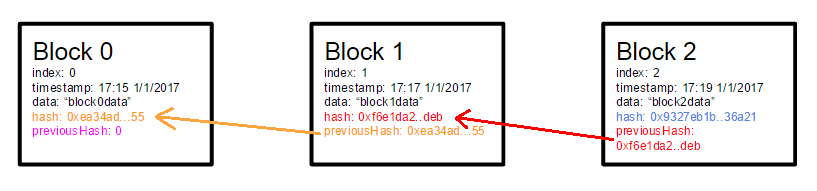
\includegraphics[scale=0.4]{blockchain_scheme}
	\caption{Структура блоков в блокчейне.}
	\label{fig:blockchain_scheme}
\end{figure}



\begin{thebibliography}{9}

	\bibitem{lamport94}
	  \emph{Как работает Эфириум (Ethereum)?}
	  https://habr.com/post/407583/

\end{thebibliography}

\end{document}